%&preformat-present

\newif\ifpresentation % Условие, проверяющее, что документ --- презентация
\presentationtrue
\documentclass[10pt, xcolor={dvipsnames, table, hyperref}]{beamer}

%%% Добавление поясняющих записей (notes) к презентации %%%
\makeatletter
\@ifundefined{c@presnotes}{
    \newcounter{presnotes}
    \setcounter{presnotes}{0}       % 0 --- выкл;
                                    % 1 --- вкл, записи на отдельном слайде;
                                    % 2 --- вкл, записи на основном слайде;
}{}
\makeatother

%%% Положение поясняющих записей (notes) при значении presnotes=2 %%%
\newcommand{\presposition}{left}  % возможные значения: left, right, top, bottom

%%% Добавление логотипа из файла images/logo на первом слайде %%%
\makeatletter
\@ifundefined{c@logotitle}{
    \newcounter{logotitle}
    \setcounter{logotitle}{1}       % 0 --- выкл;
                                    % 1 --- вкл
}{}
\makeatother

%%% Добавление логотипа из файла images/logo на слайдах (кроме первого и последнего) %%%
\makeatletter
\@ifundefined{c@logoother}{
    \newcounter{logoother}
    \setcounter{logoother}{0}       % 0 --- выкл;
                                    % 1 --- вкл
}{}
\makeatother

\setcounter{MaxMatrixCols}{20}               % Общие настройки шаблона
%%% Проверка используемого TeX-движка %%%
\newif\ifxetexorluatex   % определяем новый условный оператор (http://tex.stackexchange.com/a/47579)
\ifxetex
    \xetexorluatextrue
\else
    \ifluatex
        \xetexorluatextrue
    \else
        \xetexorluatexfalse
    \fi
\fi

\newif\ifsynopsis           % Условие, проверяющее, что документ --- автореферат

\usepackage{etoolbox}[2015/08/02]               % Для продвинутой проверки разных условий
\providebool{presentation}

%%% Поля и разметка страницы %%%
\usepackage{pdflscape}                              % Для включения альбомных страниц
\usepackage{geometry}                               % Для последующего задания полей

%%% Математические пакеты %%%
\usepackage{amsthm,amsmath,amscd}   % Математические дополнения от AMS
\usepackage{amsfonts,amssymb}       % Математические дополнения от AMS
\usepackage{mathtools}              % Добавляет окружение multlined
\usepackage{xfrac}                  % Красивые дроби
\usepackage[
    locale = DE,
    list-separator       = {;\,},
    list-final-separator = {;\,},
    list-pair-separator  = {;\,},
    range-phrase={\text{\ensuremath{-}}},
    % quotient-mode        = fraction, % красивые дроби могут не соответствовать ГОСТ
    fraction-function    = \sfrac,
    separate-uncertainty,
    ]{siunitx}                      % Размерности SI
\sisetup{inter-unit-product = \ensuremath{{}\cdot{}}}

% Кириллица в нумерации subequations
% Для правильной работы требуется выполнение сразу после загрузки пакетов
\patchcmd{\subequations}{\def\theequation{\theparentequation\alph{equation}}}
{\def\theequation{\theparentequation\asbuk{equation}}}
{\typeout{subequations patched}}{\typeout{subequations not patched}}

%%%% Установки для размера шрифта 14 pt %%%%
%% Формирование переменных и констант для сравнения (один раз для всех подключаемых файлов)%%
%% должно располагаться до вызова пакета fontspec или polyglossia, потому что они сбивают его работу
\newlength{\curtextsize}
\newlength{\bigtextsize}
\setlength{\bigtextsize}{13.9pt}

\makeatletter
%\show\f@size                                       % неплохо для отслеживания, но вызывает стопорение процесса, если документ компилируется без команды  -interaction=nonstopmode
\setlength{\curtextsize}{\f@size pt}
\makeatother

%%% Кодировки и шрифты %%%
\ifxetexorluatex
    \PassOptionsToPackage{no-math}{fontspec}        % https://tex.stackexchange.com/a/26295/104425
    \usepackage{polyglossia}[2014/05/21]            % Поддержка многоязычности (fontspec подгружается автоматически)
\else
   %%% Решение проблемы копирования текста в буфер кракозябрами
    \ifnumequal{\value{usealtfont}}{0}{}{
        \input glyphtounicode.tex
        \input glyphtounicode-cmr.tex %from pdfx package
        \pdfgentounicode=1
    }
    \usepackage{cmap}                               % Улучшенный поиск русских слов в полученном pdf-файле
    \ifnumequal{\value{usealtfont}}{2}{}{
        \defaulthyphenchar=127                      % Если стоит до fontenc, то переносы не впишутся в выделяемый текст при копировании его в буфер обмена
    }
    \usepackage{textcomp}
    \usepackage[T1,T2A]{fontenc}                    % Поддержка русских букв
    \ifnumequal{\value{usealtfont}}{1}{% Используется pscyr, при наличии
        \IfFileExists{pscyr.sty}{\usepackage{pscyr}}{}  % Подключение pscyr
    }{}
    \usepackage[utf8]{inputenc}[2014/04/30]         % Кодировка utf8
    \usepackage[english, russian]{babel}[2014/03/24]% Языки: русский, английский
    \ifnumequal{\value{usealtfont}}{2}{
        % http://dxdy.ru/post1238763.html#p1238763
        \usepackage[scaled=0.960]{XCharter}[2017/12/19] % Подключение русифицированных шрифтов XCharter
        \usepackage[charter, vvarbb, scaled=1.048]{newtxmath}[2017/12/14]
        \ifpresentation
        \else
            \setDisplayskipStretch{-0.078}
        \fi
    }{}
\fi

%%% Оформление абзацев %%%
\usepackage{indentfirst}                            % Красная строка

%%% Цвета %%%
\ifpresentation
\else
    \usepackage[dvipsnames, table, hyperref]{xcolor} % Совместимо с tikz
\fi

%%% Таблицы %%%
\usepackage{longtable,ltcaption} % Длинные таблицы
\usepackage{multirow,makecell}   % Улучшенное форматирование таблиц
\usepackage{tabu, tabulary}      % таблицы с автоматически подбирающейся
                                 % шириной столбцов (tabu обязательно
                                 % до hyperref вызывать)
\usepackage{threeparttable}      % автоматический подгон ширины подписи таблицы

%%% Общее форматирование
\usepackage{soulutf8}                               % Поддержка переносоустойчивых подчёркиваний и зачёркиваний
\usepackage{icomma}                                 % Запятая в десятичных дробях

%%% Оптимизация расстановки переносов и длины последней строки абзаца
\IfFileExists{impnattypo.sty}{% проверка установленности пакета impnattypo
    \ifluatex
        \ifnumequal{\value{draft}}{1}{% Черновик
            \usepackage[hyphenation, lastparline, nosingleletter, homeoarchy,
            rivers, draft]{impnattypo}
        }{% Чистовик
            \usepackage[hyphenation, lastparline, nosingleletter]{impnattypo}
        }
    \else
        \usepackage[hyphenation, lastparline]{impnattypo}
    \fi
}{}

%% Векторная графика

\usepackage{tikz}                   % Продвинутый пакет векторной графики
\usetikzlibrary{chains}             % Для примера tikz рисунка
\usetikzlibrary{shapes.geometric}   % Для примера tikz рисунка
\usetikzlibrary{shapes.symbols}     % Для примера tikz рисунка
\usetikzlibrary{arrows}             % Для примера tikz рисунка
\usetikzlibrary{petri,topaths,snakes}

%%% Гиперссылки %%%
\usepackage{hyperref}[2012/11/06]

%%% Изображения %%%
\usepackage{graphicx}[2014/04/25]                   % Подключаем пакет работы с графикой

%%% Счётчики %%%
\usepackage[figure,table]{totalcount}               % Счётчик рисунков и таблиц
\usepackage{totcount}                               % Пакет создания счётчиков на основе последнего номера подсчитываемого элемента (может требовать дважды компилировать документ)
\usepackage{totpages}                               % Счётчик страниц, совместимый с hyperref (ссылается на номер последней страницы). Желательно ставить последним пакетом в преамбуле

%%% Продвинутое управление групповыми ссылками (пока только формулами) %%%
\ifpresentation
\else
    \usepackage[russian]{cleveref} % cleveref имеет сложности со считыванием
    % языка из babel. Такое решение русификации вывода выбрано вместо
    % определения в documentclass из опасности что-то лишнее передать во все
    % остальные пакеты, включая библиографию.
    \creflabelformat{equation}{#2#1#3} % Формат по умолчанию ставил круглые
    % скобки вокруг каждого номера ссылки, теперь просто номера ссылок без
    % какого-либо дополнительного оформления
    \crefrangelabelformat{equation}{#3#1#4\cyrdash#5#2#6} % Интервалы в русском
    % языке принято делать через тире, если иное не оговорено

    % решение проблемы с "и" в \labelcref
    % https://tex.stackexchange.com/a/455124/104425
    \ifxetexorluatex
        \DeclareTextSymbol{\cyri}\UnicodeEncodingName{"0438} % и
    \fi

    % Добавление возможности использования пробелов в \labelcref
    % https://tex.stackexchange.com/a/340502/104425
    \usepackage{kvsetkeys}
    \makeatletter
    \let\org@@cref\@cref
    \renewcommand*{\@cref}[2]{%
        \edef\process@me{%
            \noexpand\org@@cref{#1}{\zap@space#2 \@empty}%
        }\process@me
    }
    \makeatother

    \newcommand{\eqrefs}[1]{(\labelcref{#1})}
    \newcommand{\refs}[1]{\labelcref{#1}}
\fi

\ifnumequal{\value{draft}}{1}{% Черновик
    \usepackage[firstpage]{draftwatermark}
    \SetWatermarkText{DRAFT}
    \SetWatermarkFontSize{14pt}
    \SetWatermarkScale{15}
    \SetWatermarkAngle{45}
}{}

%%% Исправление положения якорей подписей (под)рисунков %%%
% Без hypcap и патча, при клике по ссылке на подрисунок, просмотрщик pdf прыгает "к подписи" а не "к рисунку".
% Подробнее: https://github.com/AndreyAkinshin/Russian-Phd-LaTeX-Dissertation-Template/issues/238
% (!) Даже с патчем, если мешать в одной фиге разные типы подфиг (subbottom и subcaption) - ссылки всё равно будут работать неправильно  (см. https://www.overleaf.com/read/czmbmmtnqrrg ).
\ifpresentation
\else
    \usepackage[all]{hypcap}

    \makeatletter
    \ltx@ifclasslater{memoir}{2018/12/13}{
        % Предполагается, что в следующей версии класс будет исправлен
        \typeout{Assuming this version of memoir is free from the jumping-to-caption bug.}
    }{
        \usepackage{xpatch}

        \newcommand\mem@step@subcounter{\refstepcounter{sub\@captype}\@contkeep}

        \xpatchcmd{\@memsubbody}%
        {\refstepcounter{sub\@captype}\@contkeep}% search pattern
        {}% replacement
        {\typeout{@memsubbody is patched}}%
        {\typeout{@memsubbody is NOT patched}}%

        \xpatchcmd{\@memcontsubbody}%
        {\refstepcounter{sub\@captype}\@contkeep}% pattern
        {}% replacement
        {\typeout{@memcontsubbody is patched}}%
        {\typeout{@memcontsubbody is NOT patched}}%

        \xpatchcmd{\@memsubfloat}%
        {\vbox\bgroup}% search pattern
        {\vbox\bgroup\mem@step@subcounter}% replacement
        {\typeout{@memsubfloat patch is ok}}%
        {\typeout{@memsubfloat patch is NOT ok}}%

        \xpatchcmd{\subcaption}%
        {\refstepcounter{sub\@captype}}% search pattern
        {\H@refstepcounter{sub\@captype}}% replacement
        {\typeout{subcaption second patch is ok}}%
        {\typeout{subcaption second patch is NOT ok}}%
    }
    \makeatother
\fi

%%% Цитата, не приводимая в автореферате:
% возможно, актуальна только для biblatex
%\newcommand{\citeinsynopsis}[1]{\ifsynopsis\else ~\cite{#1} \fi}

% если текущий процесс запущен библиотекой tikz-external, то прекомпиляция должна быть включена
\ifdefined\tikzexternalrealjob
    \setcounter{imgprecompile}{1}
\fi

\ifnumequal{\value{imgprecompile}}{1}{% Только если у нас включена предкомпиляция
    \usetikzlibrary{external}   % подключение возможности предкомпиляции
    \tikzexternalize[prefix=images/cache/] % activate! % здесь можно указать отдельную папку для скомпилированных файлов
    \ifxetex
        \tikzset{external/up to date check={diff}}
    \fi
}{}
            % Пакеты общие для диссертации и автореферата
%%% Основные сведения %%%
\newcommand{\thesisAuthorLastName}{Лебедев}
\newcommand{\thesisAuthorOtherNames}{Олег Владимирович}
\newcommand{\thesisAuthorInitials}{О.\,В.}
\newcommand{\thesisAuthor}             % Диссертация, ФИО автора
{%
    \texorpdfstring{% \texorpdfstring takes two arguments and uses the first for (La)TeX and the second for pdf
        \thesisAuthorLastName~\thesisAuthorOtherNames% так будет отображаться на титульном листе или в тексте, где будет использоваться переменная
    }{%
        \thesisAuthorLastName, \thesisAuthorOtherNames% эта запись для свойств pdf-файла. В таком виде, если pdf будет обработан программами для сбора библиографических сведений, будет правильно представлена фамилия.
    }
}
\newcommand{\thesisAuthorShort}        % Диссертация, ФИО автора инициалами
{\thesisAuthorInitials~\thesisAuthorLastName}
% \newcommand{\thesisUdk}                % Диссертация, УДК
% {\todo{xxx.xxx}}
\newcommand{\thesisTitle}              % Диссертация, название
{Исследование и разработка имитационной модели критичного к ошибкам объекта контроля}
\newcommand{\thesisSpecialtyNumber}    % Диссертация, специальность, номер
{09.04.04}
\newcommand{\thesisSpecialtyTitle}     % Диссертация, специальность, название
{Программная инженерия}
\newcommand{\thesisDegree}             % Диссертация, ученая степень
{\todo{магистр}}
\newcommand{\thesisDegreeShort}        % Диссертация, ученая степень, краткая запись
{\todo{м.}}
\newcommand{\thesisCity}               % Диссертация, город написания диссертации
{Санкт-Петербург}
\newcommand{\thesisYear}               % Диссертация, год написания диссертации
{2021}
\newcommand{\thesisOrganization}       % Диссертация, организация
{Федеральное государственное автономное образовательное учреждение высшего образования
    «Санкт-Петербургский государственный университет аэрокосмического приборостроения»}
\newcommand{\thesisOrganizationShort}  % Диссертация, краткое название организации для доклада
{ФГАОУ ВО ГУАП}

\newcommand{\thesisInOrganization}     % Диссертация, организация в предложном падеже: Работа выполнена в ...
{\todo{ФГАОУ ВО ГУАП}}

\newcommand{\supervisorFio}            % Научный руководитель, ФИО
{Коромысличенко Владислав Николаевич}
\newcommand{\supervisorRegalia}        % Научный руководитель, регалии
{Кандидат технических наук}
\newcommand{\supervisorFioShort}       % Научный руководитель, ФИО
{В.~Н.~Коромысличенко}
\newcommand{\supervisorRegaliaShort}   % Научный руководитель, регалии
{к.\,т.\,н.}


\newcommand{\opponentOneFio}           % Оппонент 1, ФИО
{\todo{Фамилия Имя Отчество}}
\newcommand{\opponentOneRegalia}       % Оппонент 1, регалии
{\todo{доктор физико-математических наук, профессор}}
\newcommand{\opponentOneJobPlace}      % Оппонент 1, место работы
{\todo{Не очень длинное название для места работы}}
\newcommand{\opponentOneJobPost}       % Оппонент 1, должность
{\todo{старший научный сотрудник}}

\newcommand{\opponentTwoFio}           % Оппонент 2, ФИО
{\todo{Фамилия Имя Отчество}}
\newcommand{\opponentTwoRegalia}       % Оппонент 2, регалии
{\todo{кандидат физико-математических наук}}
\newcommand{\opponentTwoJobPlace}      % Оппонент 2, место работы
{\todo{Основное место работы c длинным длинным длинным длинным названием}}
\newcommand{\opponentTwoJobPost}       % Оппонент 2, должность
{\todo{старший научный сотрудник}}

\newcommand{\leadingOrganizationTitle} % Ведущая организация, дополнительные строки
{АО~<<Концерн ``МПО-Гидроприбор''>>}

\newcommand{\defenseDate}              % Защита, дата
{\todo{DD mmmmmmmm YYYY~г.~в~XX часов}}
\newcommand{\defenseCouncilNumber}     % Защита, номер диссертационного совета
{\todo{Д\,123.456.78}}
\newcommand{\defenseCouncilTitle}      % Защита, учреждение диссертационного совета
{\todo{Название учреждения}}
\newcommand{\defenseCouncilAddress}    % Защита, адрес учреждение диссертационного совета
{\todo{Адрес}}
\newcommand{\defenseCouncilPhone}      % Телефон для справок
{\todo{+7~(0000)~00-00-00}}

\newcommand{\defenseSecretaryFio}      % Секретарь диссертационного совета, ФИО
{\todo{Фамилия Имя Отчество}}
\newcommand{\defenseSecretaryRegalia}  % Секретарь диссертационного совета, регалии
{\todo{д-р~физ.-мат. наук}}            % Для сокращений есть ГОСТы, например: ГОСТ Р 7.0.12-2011 + http://base.garant.ru/179724/#block_30000

\newcommand{\synopsisLibrary}          % Автореферат, название библиотеки
{\todo{Название библиотеки}}
\newcommand{\synopsisDate}             % Автореферат, дата рассылки
{\todo{DD mmmmmmmm YYYY года}}

% To avoid conflict with beamer class use \providecommand
\providecommand{\keywords}%            % Ключевые слова для метаданных PDF диссертации и автореферата
{}
                % Основные сведения
\input{common/fonts}               % Определение шрифтов (частичное)
% Новые переменные, которые могут использоваться во всём проекте
% ГОСТ 7.0.11-2011
% 9.2 Оформление текста автореферата диссертации
% 9.2.1 Общая характеристика работы включает в себя следующие основные структурные
% элементы:
% актуальность темы исследования;
\newcommand{\actualityTXT}{Актуальность темы.}
% степень ее разработанности;
\newcommand{\progressTXT}{Степень разработанности темы.}
% цели и задачи;
\newcommand{\aimTXT}{Целью}
\newcommand{\tasksTXT}{задачи}
% научную новизну;
\newcommand{\noveltyTXT}{Научная новизна:}
% теоретическую и практическую значимость работы;
%\newcommand{\influenceTXT}{Теоретическая и практическая значимость}
% или чаще используют просто
\newcommand{\influenceTXT}{Практическая значимость}
% методологию и методы исследования;
\newcommand{\methodsTXT}{Методология и методы исследования.}
% положения, выносимые на защиту;
\newcommand{\defpositionsTXT}{Основные положения, выносимые на~защиту:}
% степень достоверности и апробацию результатов.
\newcommand{\reliabilityTXT}{Достоверность}
\newcommand{\probationTXT}{Апробация работы.}

\newcommand{\contributionTXT}{Личный вклад.}
\newcommand{\publicationsTXT}{Публикации.}


%%% Заголовки библиографии:

% для автореферата:
\newcommand{\bibtitleauthor}{Публикации автора по теме диссертации}

% для стиля библиографии `\insertbiblioauthorgrouped`
\newcommand{\bibtitleauthorvak}{В изданиях из списка ВАК РФ}
\newcommand{\bibtitleauthorscopus}{В изданиях, входящих в международную базу цитирования Scopus}
\newcommand{\bibtitleauthorwos}{В изданиях, входящих в международную базу цитирования Web of Science}
\newcommand{\bibtitleauthorother}{В прочих изданиях}
\newcommand{\bibtitleauthorconf}{В сборниках трудов конференций}

% для стиля библиографии `\insertbiblioauthorimportant`:
\newcommand{\bibtitleauthorimportant}{Наиболее значимые \protect\MakeLowercase\bibtitleauthor}

% для списка литературы в диссертации и списка чужих работ в автореферате:
\newcommand{\bibtitlefull}{Список литературы} % (ГОСТ Р 7.0.11-2011, 4)

% Название программы на французский манер.
\newcommand{\protege}{\texttt{Protégé}\xspace}

% Название компонентов онтологии
\newcommand{\mbelement}{\texttt{Modbus\-Ele\-ment}\xspace}
\newcommand{\mbdata}{\texttt{Modbus\-Data}\xspace}
\newcommand{\mbreader}{\texttt{IModbus\-Ele\-ment\-Rea\-der}\xspace}
\newcommand{\mbwriter}{\texttt{IModbus\-Ele\-ment\-Wri\-ter}\xspace}
\newcommand{\mbrelationed}{\texttt{Modbus\-Data\-Re\-la\-tioned}\xspace}
\newcommand{\mbdevice}{\texttt{IDevice\-Wri\-ter}\xspace}

% Разделители типов данных в RDF схеме
\newcommand{\rdfwedge}{${}^{\wedge\wedge}$}

%%% Добавление поясняющих записей (notes) к презентации %%%
\makeatletter
\@ifundefined{c@presnotes}{
    \newcounter{presnotes}
    \setcounter{presnotes}{0}       % 0 --- выкл;
                                    % 1 --- вкл, записи на отдельном слайде;
                                    % 2 --- вкл, записи на основном слайде;
}{}
\makeatother

%%% Положение поясняющих записей (notes) при значении presnotes=2 %%%
\newcommand{\presposition}{left}  % возможные значения: left, right, top, bottom

%%% Добавление логотипа из файла images/logo на первом слайде %%%
\makeatletter
\@ifundefined{c@logotitle}{
    \newcounter{logotitle}
    \setcounter{logotitle}{1}       % 0 --- выкл;
                                    % 1 --- вкл
}{}
\makeatother

%%% Добавление логотипа из файла images/logo на слайдах (кроме первого и последнего) %%%
\makeatletter
\@ifundefined{c@logoother}{
    \newcounter{logoother}
    \setcounter{logoother}{0}       % 0 --- выкл;
                                    % 1 --- вкл
}{}
\makeatother

\setcounter{MaxMatrixCols}{20}         % Настройки презентации
\hypersetup{
    unicode=true,          % non-Latin characters in Acrobat’s bookmarks
}
\usepackage{mathtext}
\usepackage{enumerate,float,indentfirst}
\usepackage{appendixnumberbeamer} % не считать номера страниц после команды \appendix
\usepackage{array, booktabs} % для таблиц
\usepackage{pgfpages}
\usepackage{esint} % various fancy integral symbols

\graphicspath{{images/}{Presentation/images/}{Dissertation/images/}} % папки с графикой

\DeclareRobustCommand{\todo}{\textcolor{red}}       % решаем проблему превращения названия цвета в результате \MakeUppercase, http://tex.stackexchange.com/a/187930, \DeclareRobustCommand protects \todo from expanding inside \MakeUppercase

\makeatletter
\newcommand*{\rom}[1]{\expandafter\@slowromancap\romannumeral#1@}
\makeatother

\newcommand{\itemi}{\item[\checkmark]}

\usepackage{tkz-berge}  % Библиотеки презентации
% Общие стили оформления.
% Возможные варианты значений ищите в описании библиотеки beamer
\usetheme{Pittsburgh}
\usecolortheme{whale}

% \usetheme[secheader]{Boadilla}
% \usecolortheme{seahorse}

% выключение кнопок навигации
\beamertemplatenavigationsymbolsempty

% Размеры шрифтов
\setbeamerfont{title}{size=\large}
\setbeamerfont{subtitle}{size=\small}
\setbeamerfont{author}{size=\normalsize}
\setbeamerfont{institute}{size=\small}
\setbeamerfont{date}{size=\normalsize}
\setbeamerfont{bibliography item}{size=\small}
\setbeamerfont{bibliography entry author}{size=\small}
\setbeamerfont{bibliography entry title}{size=\small}
\setbeamerfont{bibliography entry location}{size=\small}
\setbeamerfont{bibliography entry note}{size=\small}
% Аналогично можно настроить и другие размеры.
% Названия классов элементов можно найти здесь
% http://www.cpt.univ-mrs.fr/~masson/latex/Beamer-appearance-cheat-sheet.pdf

% Цвет элементов
\setbeamercolor{footline}{fg=blue}
\setbeamercolor{bibliography item}{fg=black}
\setbeamercolor{bibliography entry author}{fg=black}
\setbeamercolor{bibliography entry title}{fg=black}
\setbeamercolor{bibliography entry location}{fg=black}
\setbeamercolor{bibliography entry note}{fg=black}
% Аналогично можно настроить и другие цвета.
% Названия классов элементов можно найти здесь
% http://www.cpt.univ-mrs.fr/~masson/latex/Beamer-appearance-cheat-sheet.pdf

% Убрать иконки перед списком литературы
% https://tex.stackexchange.com/a/124271/104425
\setbeamertemplate{bibliography item}{}

% Использовать шрифт с засечками для формул
% https://tex.stackexchange.com/a/34267/104425
\usefonttheme[onlymath]{serif}

% https://tex.stackexchange.com/a/291545/104425
\makeatletter
\def\beamer@framenotesbegin{% at beginning of slide
    \usebeamercolor[fg]{normal text}
    \gdef\beamer@noteitems{}%
    \gdef\beamer@notes{}%
}
\makeatother

% footer презентации
\setbeamertemplate{footline}{
    \leavevmode%
    \hbox{%
        \begin{beamercolorbox}[wd=.333333\paperwidth,ht=2.25ex,dp=1ex,center]{}%
            % И. О. Фамилия, Организация кратко
            \thesisAuthorShort, \thesisOrganizationShort
        \end{beamercolorbox}%
        \begin{beamercolorbox}[wd=.333333\paperwidth,ht=2.25ex,dp=1ex,center]{}%
            % Город, 20XX
            \thesisCity, \thesisYear
        \end{beamercolorbox}%
        \begin{beamercolorbox}[wd=.333333\paperwidth,ht=2.25ex,dp=1ex,right]{}%
            Стр. \insertframenumber{} из \inserttotalframenumber \hspace*{2ex}
        \end{beamercolorbox}}%
    \vskip0pt%
}

% вывод на экран заметок к презентации
\ifnumequal{\value{presnotes}}{0}{}{
    \setbeameroption{show notes}
    \ifnumequal{\value{presnotes}}{2}{
        \setbeameroption{show notes on second screen=\presposition}
    }{}
}

\lstdefinelanguage{MyXML}
{
    stepnumber=1,
    keepspaces=false,
    morestring=[s][\color{brown}]{"}{"},
    morestring=[s][\color{black}]{>}{<},
    morecomment=[s]{<?}{?>},
    morecomment=[s][\color{dkgreen}]{<!--}{-->},
    stringstyle=\color{black},
    identifierstyle=\color{blue},
    keywordstyle=\color{red},
    breakatwhitespace=true,
    showspaces=false,
    showstringspaces=false,
    morekeywords={xmlns,xsi,noNamespaceSchemaLocation,type,id,x,y,%
    source,target,version,tool,transRef,roleRef,%
    objective,eventually}
}

\lstdefinelanguage{sparql}%
{%
    stepnumber=1,%
    morecomment=[l][\color{gray}]{\#},
    morecomment=[n][\color{gray}\small]{<http}{\#>},
    morestring=[b][\color{OliveGreen}]{\"},
    % variables
    keywordsprefix=?,
    classoffset=0,
    keywordstyle=\color{Sepia},
    morekeywords={},
    % prefixes
    classoffset=1,
    keywords={rdf,rdfs,owl,xsd,purl,anpa},
    keywordstyle=\color{Purple},
    % keywords
    classoffset=2,
    keywords={SELECT,CONSTRUCT,DESCRIBE,ASK,WHERE,FROM,NAMED,PREFIX,BASE,OPTIONAL,
              FILTER,GRAPH,LIMIT,OFFSET,SERVICE,UNION,EXISTS,NOT,BINDINGS,MINUS},
    keywordstyle=\color{blue}\textmd,
}

%решаем проблему с кириллицей в комментариях (в pdflatex) https://tex.stackexchange.com/a/103712
\lstset{extendedchars=true,keepspaces=true,literate={Ö}{{\"O}}1
    {Ä}{{\"A}}1
    {Ü}{{\"U}}1
    {ß}{{\ss}}1
    {ü}{{\"u}}1
    {ä}{{\"a}}1
    {ö}{{\"o}}1
    {~}{{\textasciitilde}}1
    {а}{{\selectfont\char224}}1
    {б}{{\selectfont\char225}}1
    {в}{{\selectfont\char226}}1
    {г}{{\selectfont\char227}}1
    {д}{{\selectfont\char228}}1
    {е}{{\selectfont\char229}}1
    {ё}{{\"e}}1
    {ж}{{\selectfont\char230}}1
    {з}{{\selectfont\char231}}1
    {и}{{\selectfont\char232}}1
    {й}{{\selectfont\char233}}1
    {к}{{\selectfont\char234}}1
    {л}{{\selectfont\char235}}1
    {м}{{\selectfont\char236}}1
    {н}{{\selectfont\char237}}1
    {о}{{\selectfont\char238}}1
    {п}{{\selectfont\char239}}1
    {р}{{\selectfont\char240}}1
    {с}{{\selectfont\char241}}1
    {т}{{\selectfont\char242}}1
    {у}{{\selectfont\char243}}1
    {ф}{{\selectfont\char244}}1
    {х}{{\selectfont\char245}}1
    {ц}{{\selectfont\char246}}1
    {ч}{{\selectfont\char247}}1
    {ш}{{\selectfont\char248}}1
    {щ}{{\selectfont\char249}}1
    {ъ}{{\selectfont\char250}}1
    {ы}{{\selectfont\char251}}1
    {ь}{{\selectfont\char252}}1
    {э}{{\selectfont\char253}}1
    {ю}{{\selectfont\char254}}1
    {я}{{\selectfont\char255}}1
    {А}{{\selectfont\char192}}1
    {Б}{{\selectfont\char193}}1
    {В}{{\selectfont\char194}}1
    {Г}{{\selectfont\char195}}1
    {Д}{{\selectfont\char196}}1
    {Е}{{\selectfont\char197}}1
    {Ё}{{\"E}}1
    {Ж}{{\selectfont\char198}}1
    {З}{{\selectfont\char199}}1
    {И}{{\selectfont\char200}}1
    {Й}{{\selectfont\char201}}1
    {К}{{\selectfont\char202}}1
    {Л}{{\selectfont\char203}}1
    {М}{{\selectfont\char204}}1
    {Н}{{\selectfont\char205}}1
    {О}{{\selectfont\char206}}1
    {П}{{\selectfont\char207}}1
    {Р}{{\selectfont\char208}}1
    {С}{{\selectfont\char209}}1
    {Т}{{\selectfont\char210}}1
    {У}{{\selectfont\char211}}1
    {Ф}{{\selectfont\char212}}1
    {Х}{{\selectfont\char213}}1
    {Ц}{{\selectfont\char214}}1
    {Ч}{{\selectfont\char215}}1
    {Ш}{{\selectfont\char216}}1
    {Щ}{{\selectfont\char217}}1
    {Ъ}{{\selectfont\char218}}1
    {Ы}{{\selectfont\char219}}1
    {Ь}{{\selectfont\char220}}1
    {Э}{{\selectfont\char221}}1
    {Ю}{{\selectfont\char222}}1
    {Я}{{\selectfont\char223}}1
    {і}{{\selectfont\char105}}1
    {ї}{{\selectfont\char168}}1
    {є}{{\selectfont\char185}}1
    {ґ}{{\selectfont\char160}}1
    {І}{{\selectfont\char73}}1
    {Ї}{{\selectfont\char136}}1
    {Є}{{\selectfont\char153}}1
    {Ґ}{{\selectfont\char128}}1
}

\useinnertheme{circles}
\newcommand{\firstcolor}{Bittersweet}
\newcommand{\secondcolor}{BurntOrange}
\newcommand{\thirdcolor}{Salmon}
\newenvironment{firstenv}{\only{\setbeamercolor{local structure}{fg=\firstcolor}}}{}
\newenvironment{secondenv}{\only{\setbeamercolor{local structure}{fg=\secondcolor}}}{}
\newenvironment{thirdenv}{\only{\setbeamercolor{local structure}{fg=\thirdcolor}}}{}        % Стили презентации
\input{Presentation/title}         % Настройки заглавной странице

%%% Библиография. Выбор движка для реализации %%%
\ifnumequal{\value{bibliosel}}{0}{%
    \input{biblio/predefined}   % Встроенная реализация с загрузкой файла через движок bibtex8
}{
    \input{biblio/biblatex}     % Реализация пакетом biblatex через движок biber
}

% Вывести информацию о версиях используемых библиотек в лог сборки
\listfiles

\begin{document}
\begin{frame}[noframenumbering,plain]
    \setcounter{framenumber}{1}
    \begin{center}
        {\thesisOrganization}
    \end{center}
    
    \begin{center}
        \vspace{10mm}\textbf{\thesisTitle}
    \end{center}
    
    \begin{flushright}
        \vspace{5mm}\emph{Работу выполнил:}\\магистрант 2 года, гр. Z8430М\\
        Лебедев О. В.\\%
        \emph{Научный руководитель:}\\
        к.т.н. Коромысличенко В. Н.
    \end{flushright}
    
    \begin{center}
        \vspace{20mm}\small{Санкт-Петербург, 2021}
    \end{center}
\end{frame}


\section{Цели и задачи}
\begin{frame}{Цели и задачи}

    \textbf{Цель:}
        разработка программного обеспечения имитатора абонентов промышленной сети Modbus
        на основе онтологической модели критичного к ошибкам объекта контроля,
        унифицированного способа представления субъектно-ориентированного механизма изменения параметров,
        для имитации как внешнего окружения так и внутреннего состояния объекта
        контроля на основе онтологической модели необитаемого подводного аппарата.

    \textbf{Задачи}:
    \begin{enumerate}
        \item произвести декомпозицию модели объекта контроля предметной области для выделения метаклассов;
        \item создать онтологическую модель предметной области;
        \item создать и отладить программное обеспечение на основе онтологической модели;
        \item внедрить в жизненный цикл разработки программного обеспечения \textit{автоматизированных систем контроля и диагностики}
              вновь созданное программное обеспечение имитатора абонентов промышленной сети Modbus.
    \end{enumerate}
\end{frame}
\note{
    \todo{Не слишком ли большая цель?\ldots}

    Основная задача моего подразделения проектирование и разработка 
    аппаратно-программных комплексов проверки технического состояния объектов контроля критичных к ошибкам.
}

\begin{frame}{Практическая значимость}

    \textbf{Актуальность}:
    \begin{itemize}
        \item Риски с комплектующими и дополнительные \rouble.
        \item Прототипирование и отладка системы контроля (СК).
        \item Сокращение сроков разработки СК.
        \item Демонстрация заказчику ПО СК.
        \item Объект контроля (ОК) отсутствует.
        \item Дорогое время работы с ОК.
        \item Разрушение ОК на граничных значениях алгоритма.
        \item Риск для жизни работников.
    \end{itemize}
\end{frame}
      % Первые слайды презентации
\section{Модель}\subsection{СК и ОК}
\begin{frame}{Модели системы и объекта контроля}{Предметная область}
    \begin{minipage}[t]{0.57\linewidth}
        \textbf{\tiny Рабочее место}
        \center{\includegraphics<1->[width=1\linewidth,keepaspectratio]{scheme_presentation}}
    \end{minipage}
    \hfill
    \begin{minipage}[t]{0.4\linewidth}
        \begin{itemize}
            \item[АНПА] автономный необитаемый подводный аппарат
            \item[АРМ] автоматизированное рабочее место
            \item[БГР] блок гальванической развязки
            \item[ОК]  объект контроля
            \item[ПЛК] программируемый логический контроллер
            \item[СК]  система контроля            
        \end{itemize}
    \end{minipage}\pause
    \vspace{3pt}
    \centering{\fbox{\parbox{.8\textwidth}{АНПА предназначен для поиска скоплений \textit{планктона},
                \textit{рыбных косяков} или \textit{китов} путем анализа испущенной специализированной зондирующей посылки.}}}
    % \centering{\leadingOrganizationTitle}
\end{frame}





\subsection{Общесистемные сущности модели}
\begin{frame}{Общесистемные сущности модели АНПА}{Объекты --- Функции --- Действия. Имитируемые сигналы}
    \vspace{-5mm}{\tiny\begin{equation*}\begin{split}
        C_1 = &A \times B,\qquad
        C_2 = \begin{pmatrix} \sum_{j=1}^l c_{1\,1j} \\ \ldots \\ \sum_{j=1}^l c_{1\,mj} \end{pmatrix},\qquad
        C_3 = \frac{C_2}{l},{}\\
        \left. C_3^* \right|_{l \equiv 6} = &
                 \left( 0.67\;\; 0.67\;\; \textcolor{\thirdcolor}{1.33}\;\; 0.67\;\; \textcolor{\thirdcolor}{1.33}\;\; 0.67\;\; 0.83\;\; 0.83\;\; 
                        0.33\;\; \textcolor{\secondcolor}{1.5}\;\;\textcolor{\secondcolor}{1.5}\;\; 0.67\;\; \textcolor{\firstcolor}{2.00}\;\; 0.67 \right)^T\,.
    \end{split}\end{equation*}}
    \textbf{Общесистемные сущности при $K_{min} = \overline{C_3^*} = 0.98$}:
    \begin{itemize}
        \item<first@1->[2.0]  блок управления батареей;
        \item<second@1->[1.5] рулевые машинки, рулевой привод;
        \item<third@1->[1.33] анализатор приемо-излучательного тракта СПО и установщик~курса.
    \end{itemize}
    %
    \hrule{}\begin{enumerate}
        \item<2-> Внешние
        \begin{itemize}
            \item<2->[Глубина] $h = \{h_1, h_2, \ldots\, h_n\} = \{F(\vec p(t); t_1), F(\vec p(t); t_2), \ldots, F(\vec p(t); t_n)\}$;
            \item<3->[Эхо-сигнал] $s_j \Rightarrow \{r_j\} \cup \{e_j\} \ne \emptyset:\,\{r_j\} \cap \{e_j\} = \emptyset$,
                где $\{e_j\}$ -- авария.
        \end{itemize}\vspace{5pt}
        \item<2-> Внутренние
        \begin{itemize}
            \item<4->[Напряжения] $U_i = \{U_1, U_2, \ldots, U_j\};\quad U_i \in [U_i^{min}, U_i^{max}]$,
            \item<4->[Токи] $I_\Sigma = \sum_k^N I_k + \hat I;\quad I_k \in [I_k^{min}, I_k^{max}];\quad \hat I \in [\hat I^{min}, \hat I^{max}]$;
            \item<5->[СУД] $\langle f; Q \rangle$ вращения вала \textit{двигателя} в виде ШИМ сигнала;
            \item<6->[Руление] $\langle s_j, \{r_j\} \rangle \Rightarrow \omega_i = \omega_i(s_j, \{r_j\})$.
        \end{itemize}    
    \end{enumerate}
\end{frame}






\section{Онтология}
\begin{frame}{Онтология модели АНПА}{\protege}
    \begin{center}

        {\huge Онтология} --- это способ показать свойства предметной области и то, как они связаны,
            определив набор понятий и категорий, которые представляют предмет.
    \end{center}
\end{frame}






\section{Реализация}\subsection{Таксономия классов}
\begin{frame}{Таксономия классов}
    \vspace{-1mm}\hspace{-5mm}\begin{minipage}[c]{0.4\linewidth}
        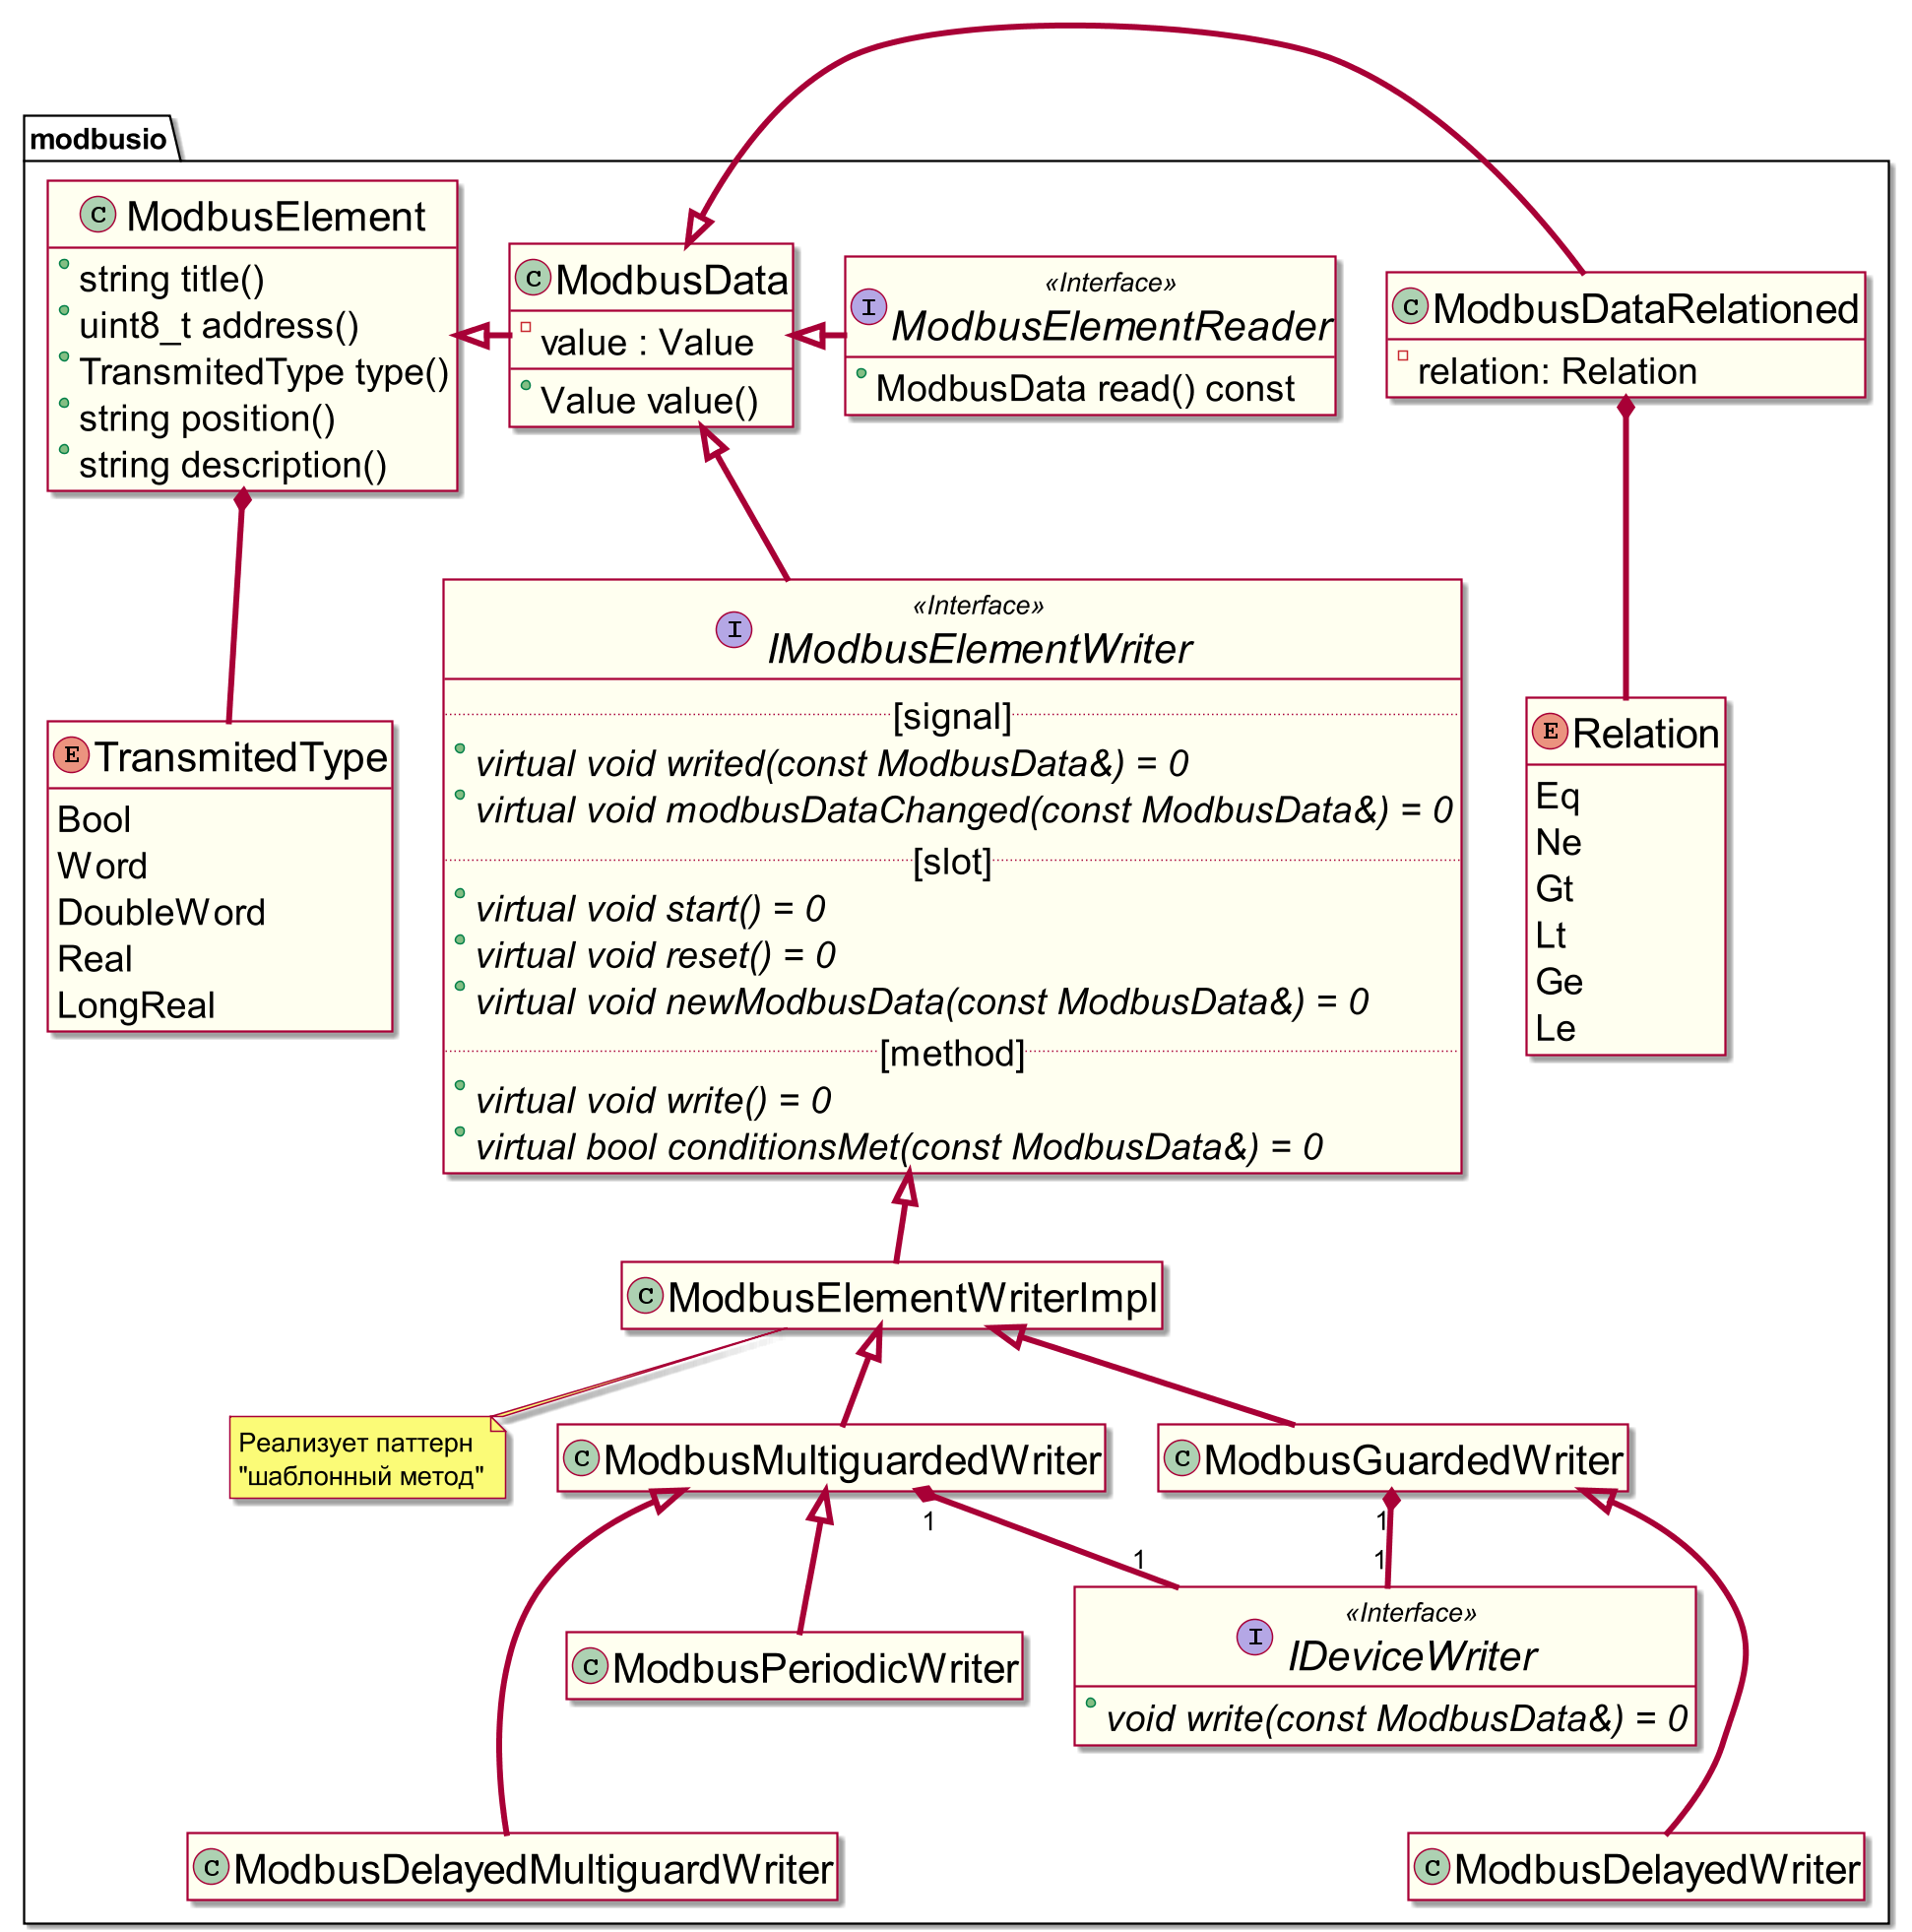
\includegraphics[height=.8\textheight]{modbus_class_relationship_short.png}
    \end{minipage}
    %
    \hspace{25mm}\begin{minipage}[c]{0.4\linewidth}
    {\tiny\begin{enumerate}
        \item \texttt{ModbusElement}, \texttt{TransmitedType}
        \item \texttt{ModbusData}, \texttt{ModbusDataRelationed} \eqref{eq:relation}
        \item Интерфейс~\texttt{IModbusElementWriter}
        \begin{itemize}
            \item {\tiny сигналы о записи и изменении}
            \item {\tiny слоты на запуск, останов и обработку новых данных}
            \item {\tiny проверка условий, запись}
        \end{itemize}
        \item Реализации интерфейса
        \item Делегирование интерфейсу \texttt{IDeviceWriter}
    \end{enumerate}}
\end{minipage}
    \begin{equation}\label{eq:relation}
        \mathcal{A} \left(\mathcal{M}_i;\, r \right) = a \in \{0, 1\}\,, \qquad
        r \in \{\equiv,\ne,>,<,\ge,\le\}
    \end{equation}
\end{frame}





\subsection{Алгоритм работы имитатора}
\begin{frame}{Алгоритм работы имитатора}
    \begin{center}
        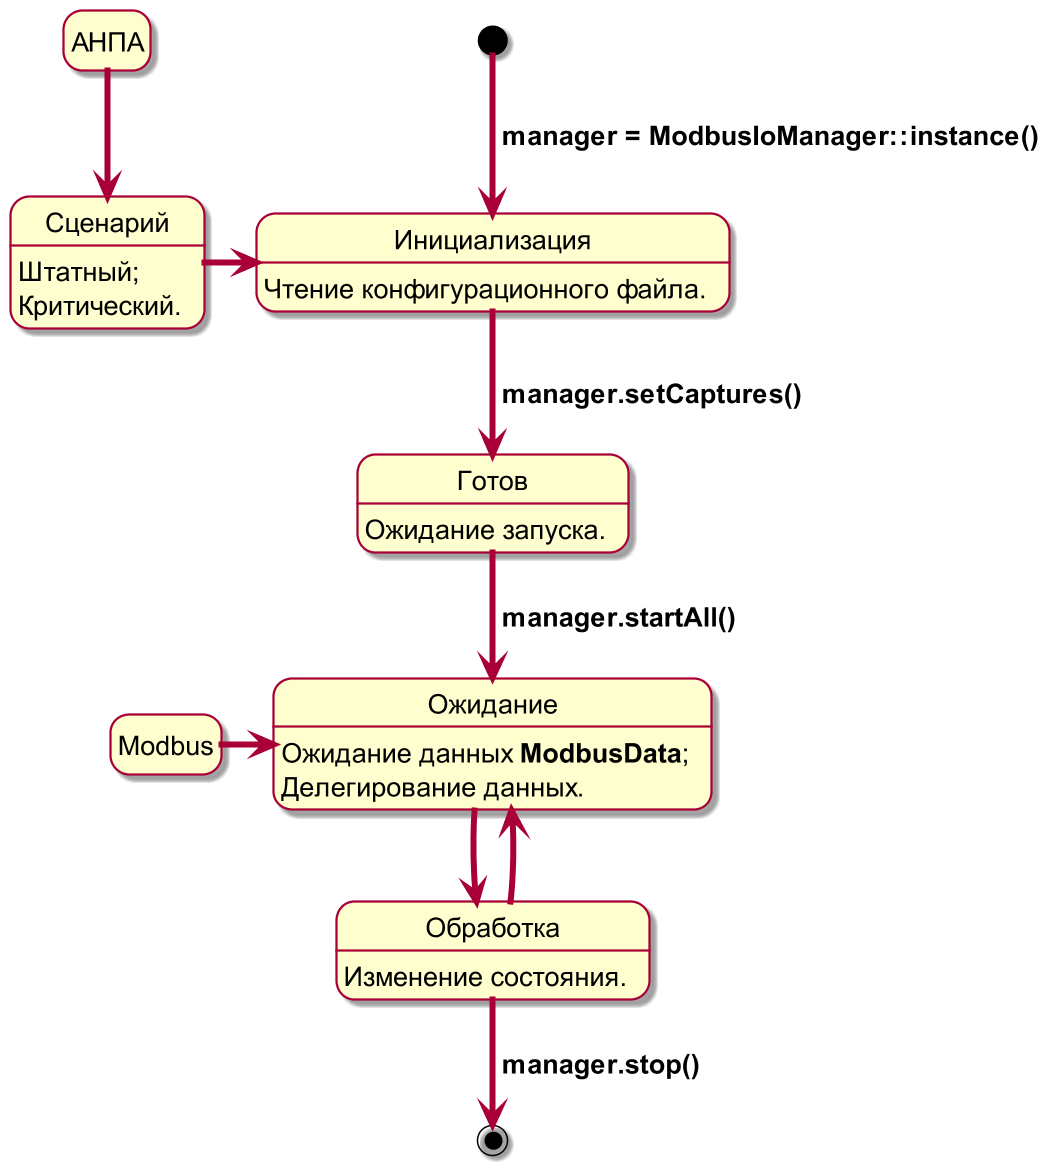
\includegraphics[height=.8\textheight]{modbusiomanager_state_diagram.png}
    \end{center}
\end{frame}






\subsection{Сценарий}
\begin{frame}{Формирование сценария}
    \textbf{Настройка:}
    \begin{enumerate}
        \item Конфигурация описывается в \texttt{XML} файле.
        \item Используется схема разметки \texttt{XSD}.
    \end{enumerate}
    \textbf{Сценарий содержит:}
    \begin{enumerate}
        \item Значения по умолчанию.
        \item Правила изменения состояния.
    \end{enumerate}
\end{frame}       % Настройки заглавной странице
\section{Заключение}\subsection{Научная и практическая значимость. Перспективы}
\begin{frame}{Заключение}{Научная и практическая значимость. Перспективы}
    \textbf{Научная новизна}
    \begin{enumerate}
        \item Графоаналитический анализ модели АНПА для выявления общесистемных объектов.
        %
        \item Декомпозиция модели АНПА на основе результатов графоаналитического анализа с целью выделения метаклассов.
        %
        \item Создан программный комплекс имитатора абонентов сети Modbus.
    \end{enumerate}
    
    \textbf{Практическая значимость}
    \begin{enumerate}
        \item Апробация \leadingOrganizationTitle на предприятии.
        %
        \item Свидетельство о государственной регистрации программы для ЭВМ.
        %
        \item ПО имитатора использует те же сущности предметной области, что и ПО АСКД.
      \end{enumerate}
      
      \textbf{Перспективы}: 
      \begin{itemize}
        \item разработка \textit{тренажерного} или \textit{учебного} комплексов;
        \item приемо-сдаточные, пусконаладочные и предъявительские испытания ПО АСКД.
      \end{itemize}
\end{frame}


\subsection{Результаты}
\begin{frame}{Результаты}
    \textcolor{blue}{\tiny Лебедев, О. В. Применении парадигмы тестирования и паттернов проектирования при разработке специализированного программного
    обеспечения в ответственных областях применения [Текст] \/ О. В. Лебедев,
    В. Н. Коромысличенко \/\/ Гидроприбор. — 2019 — Т. 5, № 48 — С. 91—96.}
    \begin{figure}[h]
        \centering
        % 
\includegraphics[width=.4\linewidth]{registration.pdf}
        \fbox{\begin{minipage}[t]{0.4\linewidth}
\includegraphics[width=\linewidth]{registration.pdf}\end{minipage}}
        \fbox{\begin{minipage}[t]{0.4\linewidth}
\includegraphics[width=\linewidth]{implementation}\end{minipage}}
    \end{figure}
\end{frame}


\begin{frame}[plain, noframenumbering] % последний слайд без оформления
    \begin{center}
        \Huge
        Спасибо за внимание!
    \end{center}
\end{frame}
    % Последние слайды презентации
\appendix
\section{Взаимодействие СК и ОК}
\begin{frame}{Рабочее место}
    \begin{center}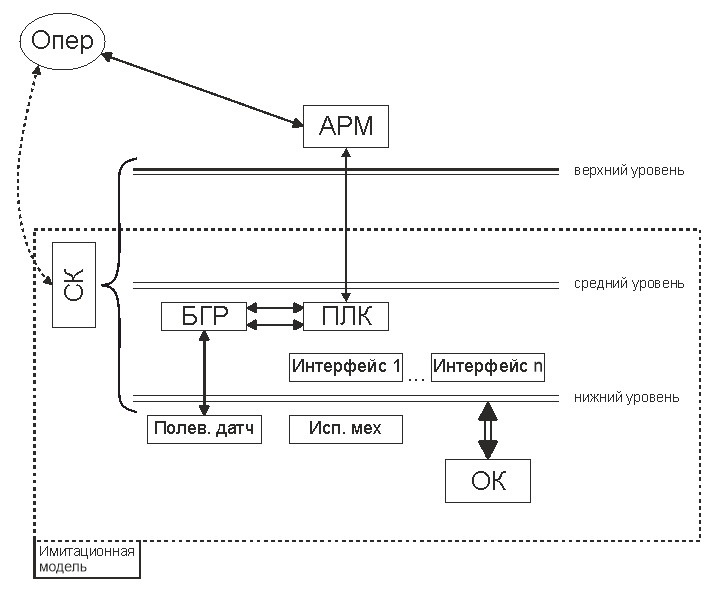
\includegraphics[height=.8\textheight,keepaspectratio]{scheme_3levels.png}\end{center}
\end{frame}



\section{Декомпозиция АНПА}
\begin{frame}{Материальная составляющая модели АНПА}{Выявление общесистемных сущностей}
    \begin{center}
    {\huge Объекты --- Функции --- Действия}\vspace{10mm}
    
    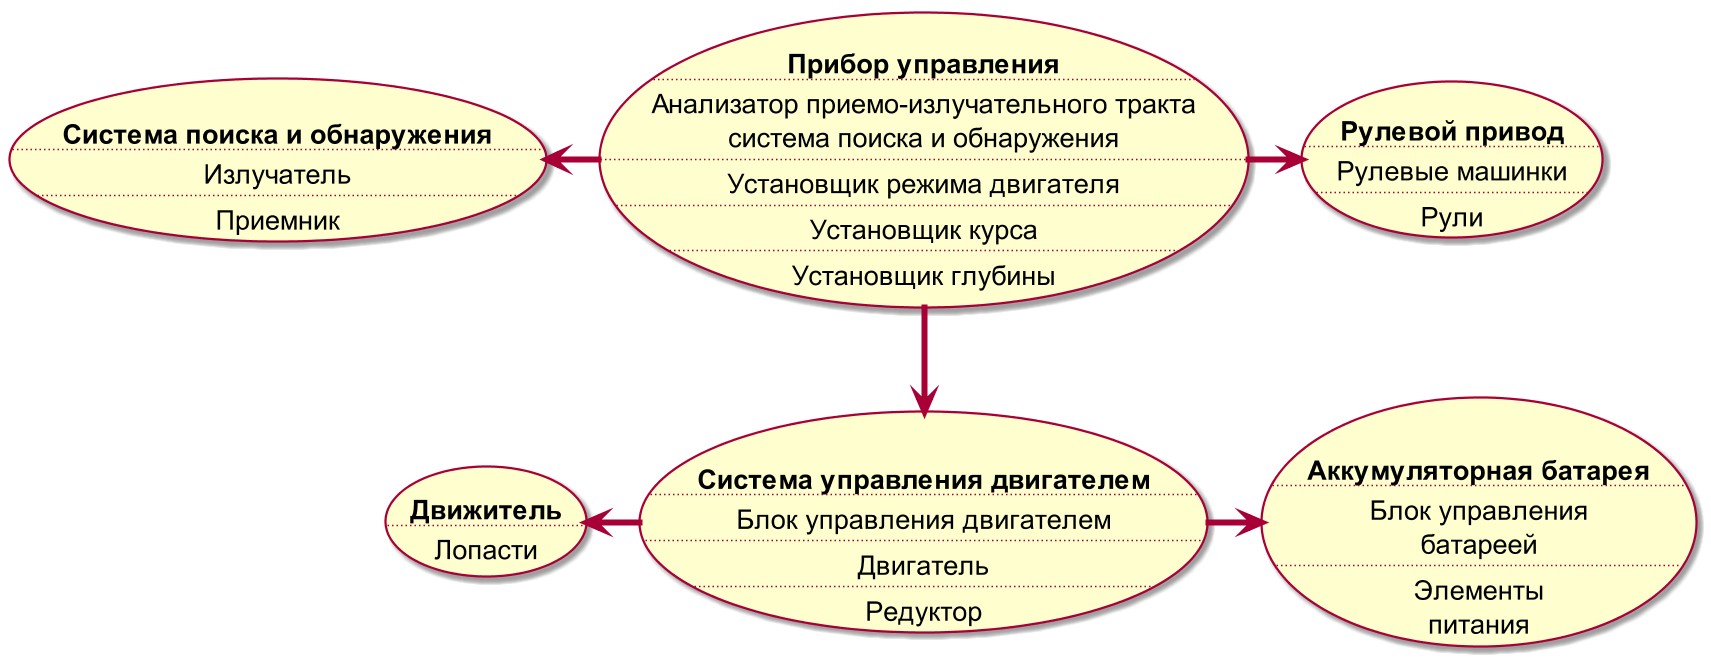
\includegraphics[width=1\linewidth,keepaspectratio]{model_anpa}\vspace{5mm}

    {\color{blue}{\noindent\tiny Елизарова, Н. Применение графоаналитического метода анализа предметной
        области при проектировании информационных систем [Текст] /
        Н. Елизарова, Е. Архангельская // Вестник ИГЭУ. — 2010 — Т. 4 — С. 5 }}

    \end{center}
\end{frame}
\note{
    Отвечаю на вопрос, а какие параметры необходимо имитировать в первую очередь --- \textbf{общесистемные}.
}

\begin{frame}{Объект -- Функция -- Действие}{\small Графоаналитический метод для выявления общесистемных сущностей.}
    {\tiny Елизарова, Н. Применение графоаналитического метода анализа предметной
    области при проектировании информационных систем [Текст] /
    Н. Елизарова, Е. Архангельская // Вестник ИГЭУ. — 2010 — Т. 4 — С. 5 }
    \tiny\begin{tabular}{cp{.2\textwidth}||c|p{.15\textwidth}||cp{.15\textwidth}}
        \toprule
        \multicolumn{2}{|c||}{\textbf{Объект}} & \multicolumn{2}{c||}{\textbf{Функции}} & \multicolumn{2}{c|}{\textbf{Действия}} \\ \midrule
        %
        \multicolumn{1}{|l|}{\multirow{2}{*}{СПО}} & Излучатель                                  & \multirow{5}{*}{Движение}          & Вперед                           & \multicolumn{1}{l|}{\multirow{3}{*}{ПУ}}  & \multicolumn{1}{l|}{Пеленгация целей}     \\ \cline{2-2} \cline{4-4} \cline{6-6}
        \multicolumn{1}{|l|}{}                     & Приемник                                    &                                    & Вправо                           & \multicolumn{1}{l|}{}                     & \multicolumn{1}{l|}{Коррекция курса}      \\ \cline{1-2} \cline{4-4} \cline{6-6}
        \multicolumn{1}{|l|}{\multirow{4}{*}{ПУ}}  & Анализатор приемо-излучательного тракта СПО &                                    & Влево                            & \multicolumn{1}{l|}{}                     & \multicolumn{1}{l|}{Коррекция глубины}    \\ \cline{2-2} \cline{4-4} \cline{5-6}
        \multicolumn{1}{|l|}{}                     & Установщик режима двигателя                 &                                    & Вверх                            & \multicolumn{1}{l|}{\multirow{2}{*}{АКБ}} & \multicolumn{1}{l|}{Хранение}             \\ \cline{2-2} \cline{4-4} \cline{6-6}
        \multicolumn{1}{|l|}{}                     & Установщик курса                            &                                    & Вниз                             & \multicolumn{1}{l|}{}                     & \multicolumn{1}{l|}{Доставка}             \\ \cline{2-6}
        \multicolumn{1}{|l|}{}                     & Установщик глубины                          & \multirow{5}{*}{Питание}           & СПО                              & \multicolumn{1}{l|}{Д}                    & \multicolumn{1}{l|}{Толкает водную среду} \\ \cline{1-2} \cline{4-6}
        \multicolumn{1}{|l|}{\multirow{3}{*}{СУД}} & БУД                                         &                                    & ПУ                               &                                           &                                           \\ \cline{2-2} \cline{4-4}
        \multicolumn{1}{|l|}{}                     & Двигатель                                   &                                    & СУД                              &                                           &                                           \\ \cline{2-2} \cline{4-4}
        \multicolumn{1}{|l|}{}                     & Редуктор                                    &                                    & РП                               &                                           &                                           \\ \cline{1-2} \cline{4-4}
        \multicolumn{1}{|l|}{\multirow{2}{*}{РП}}  & РМ                                          &                                    & Д                                &                                           &                                           \\ \cline{2-4}
        \multicolumn{1}{|l|}{}                     & Рули                                        & \multirow{2}{*}{Обнаружение}       & Излучение зондирующей посылки    &                                           &                                           \\ \cline{1-2} \cline{4-4}
        \multicolumn{1}{|l|}{Д}                    & Лопасти                                     &                                    & Прием отраженого сигнала         &                                           &                                           \\ \cline{1-4}
        \multicolumn{1}{|l|}{\multirow{2}{*}{АКБ}} & БУБ                                         & \multirow{4}{*}{Принятие решений}  & Изменить скорость движения       &                                           &                                           \\ \cline{2-2} \cline{4-4}
        \multicolumn{1}{|l|}{}                     & Модули питания                              &                                    & Изменить курс                    &                                           &                                           \\ \cline{1-2} \cline{4-4}
                                                   &                                             &                                    & Изменить глубину хода            &                                           &                                           \\ \cline{4-4}
                                                   &                                             &                                    & Изменить тип зондирующей посылки &                                           &                                           \\ \cline{3-4}
    \end{tabular}
        \begin{minipage}[t]{0.4\linewidth}
            \centering
                Матрицы связности: 
                \begin{itemize}
                    \item[$A$] взаимосвязь \textbf{Объект -- Функция} 
                    \item[$B$] взаимосвязь \textbf{Функция -- Действие} 
                    \item[$C_1 = A \times B$] взаимосвязь \textbf{Объект -- Действие} 
                \end{itemize}
        \end{minipage}
        \hfill
        \begin{minipage}[t]{0.55\linewidth}
            \vspace{1pt} $C_2 = \begin{pmatrix} \sum_{j=1}^l c_{1\,1j} \\ \ldots \\ \sum_{j=1}^l c_{1\,mj} \\ \end{pmatrix}\!; \quad C_3 = \left. \frac{C_2}{l} \right|_{l \equiv 6}$
        \end{minipage}
\end{frame}
    
\begin{frame}
    \tiny
    \begin{equation*}
        \begin{split}
        A_{16\times14} = &\begin{pmatrix}
            0 & 0 & 0 & 0 & 0 & 1 & 0 & 0 & 0 & 0 & 1 & 0 & 0 & 0 & 0 & 0 \\
            0 & 0 & 0 & 0 & 0 & 1 & 0 & 0 & 0 & 0 & 0 & 1 & 0 & 0 & 0 & 0 \\
            0 & 0 & 0 & 0 & 0 & 1 & 1 & 0 & 0 & 0 & 0 & 1 & 0 & 0 & 0 & 1 \\
            0 & 0 & 0 & 0 & 0 & 0 & 0 & 1 & 0 & 1 & 0 & 0 & 0 & 0 & 0 & 0 \\
            0 & 1 & 1 & 0 & 0 & 0 & 0 & 0 & 0 & 0 & 1 & 0 & 0 & 1 & 0 & 1 \\
            0 & 0 & 0 & 1 & 1 & 0 & 0 & 0 & 0 & 0 & 0 & 0 & 0 & 0 & 1 & 0 \\
            0 & 0 & 0 & 0 & 0 & 1 & 0 & 0 & 0 & 0 & 0 & 0 & 1 & 0 & 0 & 0 \\
            0 & 0 & 0 & 0 & 0 & 1 & 0 & 0 & 0 & 0 & 0 & 0 & 1 & 0 & 0 & 0 \\
            0 & 0 & 0 & 0 & 0 & 0 & 0 & 0 & 0 & 1 & 0 & 0 & 0 & 0 & 0 & 0 \\
            1 & 1 & 1 & 1 & 1 & 0 & 0 & 0 & 0 & 0 & 0 & 0 & 0 & 1 & 1 & 0 \\
            1 & 1 & 1 & 1 & 1 & 0 & 0 & 0 & 0 & 0 & 0 & 0 & 0 & 1 & 1 & 0 \\
            0 & 0 & 0 & 0 & 0 & 0 & 0 & 0 & 0 & 0 & 0 & 0 & 0 & 1 & 1 & 0 \\
            0 & 0 & 0 & 0 & 0 & 1 & 1 & 1 & 1 & 1 & 1 & 0 & 0 & 0 & 0 & 0 \\
            0 & 0 & 0 & 0 & 0 & 0 & 0 & 0 & 0 & 0 & 1 & 1 & 0 & 0 & 0 & 0 \\
        \end{pmatrix},{}\\
    %
        B_{6\times16} = &\begin{pmatrix}
            0 & 0 & 0 & 0 & 0 & 0 & 0 & 0 & 0 & 0 & 1 & 1 & 0 & 0 & 0 & 1 \\
            0 & 1 & 1 & 0 & 0 & 0 & 0 & 0 & 0 & 0 & 0 & 1 & 1 & 1 & 0 & 0 \\
            0 & 0 & 0 & 1 & 1 & 0 & 0 & 0 & 0 & 0 & 0 & 0 & 1 & 0 & 1 & 0 \\
            0 & 0 & 0 & 0 & 0 & 1 & 1 & 1 & 1 & 1 & 0 & 0 & 0 & 0 & 0 & 0 \\
            0 & 0 & 0 & 0 & 0 & 1 & 1 & 1 & 1 & 1 & 1 & 0 & 0 & 0 & 0 & 1 \\
            1 & 0 & 0 & 0 & 0 & 0 & 0 & 0 & 0 & 0 & 0 & 0 & 1 & 1 & 1 & 0 \\
        \end{pmatrix}^T\,,{}\\
    %
        C_1 = A \times B = &\begin{pmatrix}
            1 & 1 & 2 & 0 & 2 & 0 & 0 & 0 & 0 & 0 & 0 & 0 & 1 & 2 \\
            0 & 1 & 1 & 0 & 3 & 0 & 1 & 1 & 0 & 3 & 3 & 1 & 0 & 1 \\
            0 & 0 & 0 & 0 & 0 & 3 & 1 & 1 & 0 & 3 & 3 & 1 & 0 & 0 \\
            1 & 1 & 2 & 2 & 0 & 0 & 1 & 1 & 1 & 0 & 0 & 0 & 5 & 0 \\
            2 & 1 & 3 & 2 & 2 & 0 & 1 & 1 & 1 & 0 & 0 & 0 & 6 & 1 \\
            0 & 0 & 0 & 0 & 1 & 1 & 1 & 1 & 0 & 3 & 3 & 2 & 0 & 0 \\
        \end{pmatrix}^T_{6\times14}\,,{}\\
    %
        C_3 = &\left. \frac{C_2}{l} \right|_{l \equiv 6} = 
            \left( 0.67\;\; 0.67\;\; \textbf{1.33}\;\; 0.67\;\; \textbf{1.33}\;\; 0.67\;\; 0.83\;\; 0.83\;\; 
            0.33\;\; \textbf{1.50}\;\;\textbf{1.50}\;\; 0.67\;\; \textbf{2.00}\;\; 0.67 \right)^T\,.
    \end{split}
    \end{equation*} 

    Пороговое значение $K_{min} = \overline{C_3} = 0.98$
    \begin{itemize}
        \item[2.0]   блок управления батареей;
        \item[1.5]   рулевые машинки, рулевой привод;
        \item [1.33] анализатор приемо-излучательного тракта СПО и установщик курса.
    \end{itemize}
\end{frame}




\section{Таксономия классов}
\subsection{Графики зависимости}
\begin{frame}{Временные зависимости}{Захват значения}
    \vspace{-20mm}
    \begin{minipage}[c]{0.47\linewidth}
        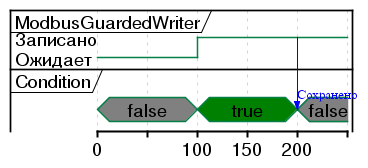
\includegraphics[width=1\linewidth]{modbus_guarded_writer}%
        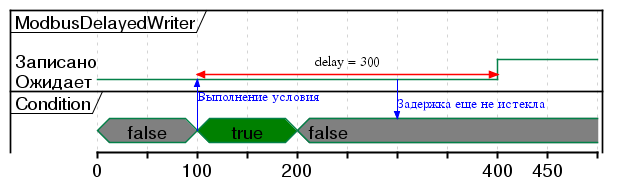
\includegraphics[width=1\linewidth]{modbus_delayed_writer}
    \end{minipage}

    \begin{minipage}[c]{0.47\linewidth}
        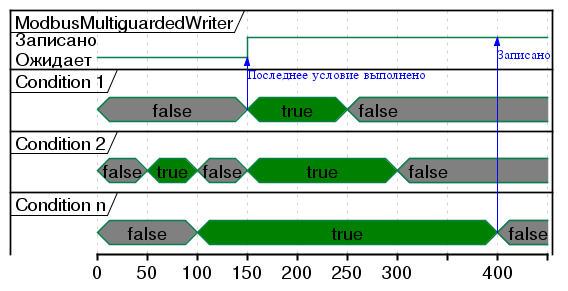
\includegraphics[width=1\linewidth]{modbus_multiguarded_writer.png}%
        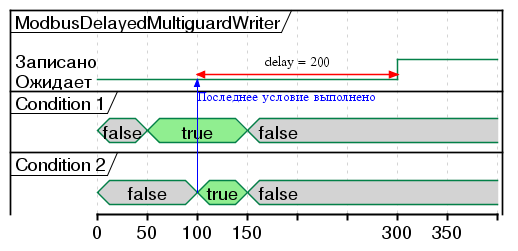
\includegraphics[width=1\linewidth]{modbus_delayed_multiguarded_writer.png}
    \end{minipage}
\end{frame}
\begin{frame}{Временные зависимости}{Захват значения}
    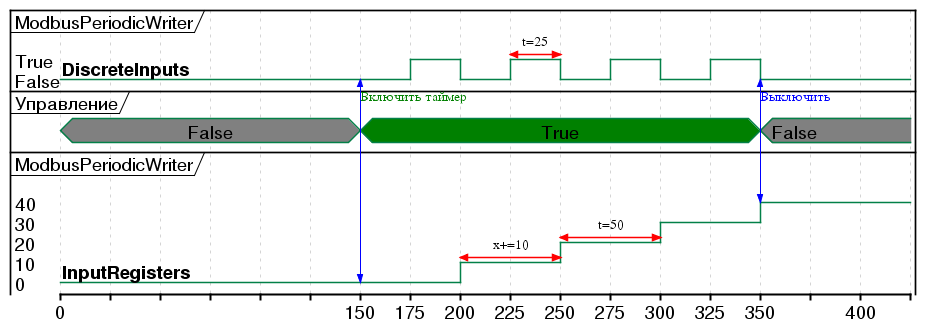
\includegraphics[width=1\linewidth]{modbus_periodic_writer.png}
\end{frame}


\subsubsection{Перегрузка методов}
\begin{frame}{Полимофизм}{Перегрузка методов}
    \hspace{-10mm}\begin{table}
        \begin{center}
        \begin{tabular}{|l|c|c|c|c|c|c||c|c|}
        \hline
            \multicolumn{1}{|c|}{\multirow{2}{*}{Наследники}} &
            \multicolumn{6}{c||}{\textbf{атрибуты}} &
            \multicolumn{2}{c|}{\textbf{override}} \\ \cline{2-9} %Переопределенные методы наследника
            \multicolumn{1}{|c|}{}     &
                \rotatebox{90}{tag} & \rotatebox{90}{value}  & \rotatebox{90}{delay}  & \rotatebox{90}{period} &
                \rotatebox{90}{delta} & \rotatebox{90}{duration} &
                \rotatebox{90}{conditionsMet} & \rotatebox{90}{newModbusData} \\ \hline
            {\tiny\texttt{ModbusGuardedWriter}}              & +    & +      & -      & -      & - &-     & + & -  \\ \hline
            {\tiny\texttt{ModbusMultiguardedWriter}}         & +    & +      & -      & -      & - &-     & + & -  \\ \hline
            {\tiny\texttt{ModbusDelayedWriter}}              & +    & +      & +      & -      & - &-     & - & +  \\ \hline
            {\tiny\texttt{ModbusDelayedMultiguardWriter}}    & +    & +      & +      & -      & - &-     & - & +  \\ \hline
            {\tiny\texttt{ModbusPeriodicWriter}}             & +    & +      & -      & +      & + &$\pm$ & + & -  \\ \hline
        \end{tabular}
        \end{center}
    \end{table}
\end{frame}


\subsection{Работа составных частей имитатора}
\begin{frame}{Жизненный цикл}
    \begin{center}
        \includegraphics<1>[width=1\linewidth]{modbus_class_components.png}
        \includegraphics<2>[height=.8\textheight]{top_level.png}
        \includegraphics<3>[height=.8\textheight]{modbuselementwriterimpl}
    \end{center}
\end{frame}


\begin{frame}{Жизненный цикл интерфейса \texttt{IModbusElementWriter}}
    \begin{center}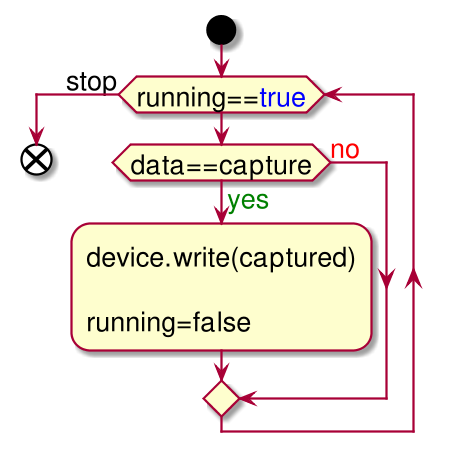
\includegraphics[height=.8\textheight]{imodbuselementwriter_activity.png}\end{center}
\end{frame}

\section{Листинги}\subsection{XML}
\begin{frame}{XML}{Мгновенная запись}
    \lstinputlisting[language=MyXML,basicstyle=\tiny]{Dissertation/listings/xml/guarded.xml}
\end{frame}
\begin{frame}{XML}{Множественные условия}
    \lstinputlisting[language=MyXML,basicstyle=\tiny]{Dissertation/listings/xml/multiguarded.xml}
\end{frame}
\begin{frame}{XML}{Запись с задержкой}
    \lstinputlisting[language=MyXML,basicstyle=\tiny]{Dissertation/listings/xml/delayed.xml}
\end{frame}
\begin{frame}{XML}{Периодическая запись}
    \lstinputlisting[language=MyXML,basicstyle=\tiny]{Dissertation/listings/xml/periodic.xml}
\end{frame}


\section{Онтология}
\subsection{Классы}
\begin{frame}{Онтология}
    \begin{center}
    \includegraphics<1>[width=.9\textwidth,keepaspectratio]{owl/anpa_hierarchy.png}
    \includegraphics<2>[width=.9\textwidth,keepaspectratio]{owl/part_of.png}
    \includegraphics<3>[width=.9\textwidth,keepaspectratio]{owl/function_movement.png}
    \end{center}
\end{frame}

\subsection{SPARQL}
\begin{frame}[fragile]{Пример SPARQL запроса}{Получение новых знаний}
    \begin{lstlisting}[language=sparql]
PREFIX anpa:<http://.../guap/ontologies/z8430m/ANPA#>
SELECT ?volt ?condition ?delay ?newvalue 
       ?relation ?condvalue ?title
WHERE { ?volt anpa:ИмеетУсловие ?condition .
    ?volt anpa:value ?newvalue .
    ?condition anpa:relation ?relation .
    ?condition anpa:title ?title .
    ?condition anpa:value ?condvalue .
    ?volt anpa:delay ?delay . FILTER (?delay > 100) . }
    \end{lstlisting}\vspace{-5mm}
    
    \begin{table}
        \begin{center}
            \begin{tabular}{cl}\hline
                volt & Uv\_пу \\\hline
                condition & C1 \\\hline
                delay & 500 \\\hline
                newvalue & 27 \\\hline
                relation & Eq \\\hline
                condvalue & true \\\hline
                title & C1 \\\hline
            \end{tabular}
        \end{center}
    \end{table}
\end{frame}


\section{GUI}
\begin{frame}{GUI}
    \begin{center}
        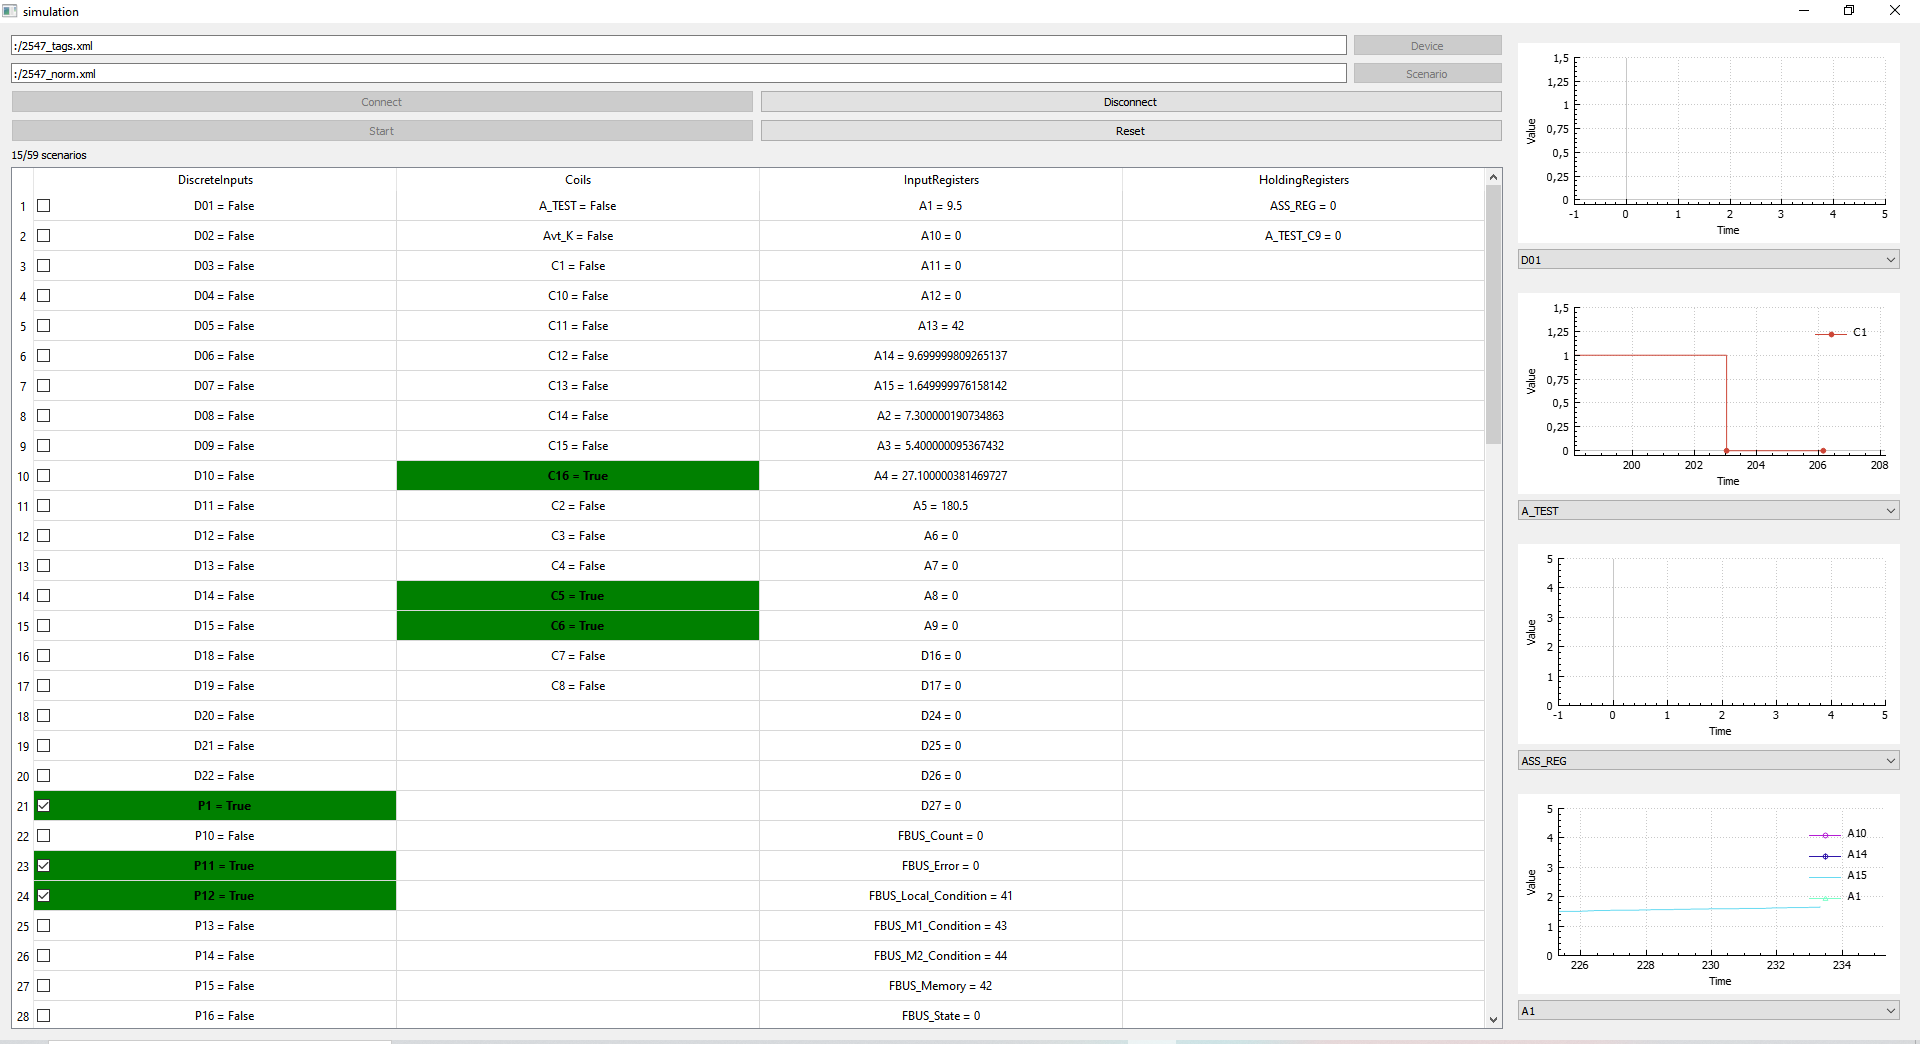
\includegraphics[width=1\linewidth]{imitator.png}
    \end{center}
\end{frame}
      % Запасные слайды презентации
\end{document}
